% ---------------------------------------------------------------------------
%  Mise en page commune des CV de Robin Canovas (français et anglais).
%  Ne se compile pas seul : compiler cv-robin-canovas.tex (FR)
%  ou cv-robin-canovas-en.tex (EN), qui chargent ce fichier.
%
%  Vérifié avec XeLaTeX (Tectonic). Sur Overleaf : Menu > Compilateur > XeLaTeX,
%  puis choisir le fichier principal (FR ou EN). Deux passes sont nécessaires
%  pour le bandeau et la colonne de droite (Overleaf, latexmk et Tectonic
%  les font tout seuls). La photo robin-canovas.jpg doit être dans le même dossier.
%
%  Lisible par les logiciels de recrutement (ATS) : texte sélectionnable,
%  police Roboto (traits d'union extraits correctement), icônes dessinées
%  en TikZ (aucun caractère parasite), pas de mots coupés, dates complètes.
% ---------------------------------------------------------------------------
\documentclass[10pt,a4paper]{article}

% Langue : le fichier principal anglais définit \cvenglish avant de charger ce fichier.
\newif\ifcvenglish
\ifdefined\cvenglish \cvenglishtrue \fi
\newcommand{\tr}[2]{\ifcvenglish#2\else#1\fi}

\usepackage[a4paper,left=12mm,right=10mm,top=10mm,bottom=6mm]{geometry}
\usepackage{iftex}
\ifPDFTeX
  \usepackage[T1]{fontenc}
  \usepackage[utf8]{inputenc}
  \input{glyphtounicode}\pdfgentounicode=1
\fi
\usepackage[sfdefault]{roboto}
\ifcvenglish
  \usepackage[english]{babel}
\else
  \usepackage[french]{babel}
  \frenchbsetup{StandardLists=true}
\fi
\usepackage[dvipsnames]{xcolor}
\usepackage{graphicx}
\usepackage{tikz}
\usetikzlibrary{babel,calc}
\usepackage{enumitem}
\usepackage{qrcode}
\usepackage[hidelinks]{hyperref}

\ifcvenglish
  \hypersetup{
    pdftitle={Resume Robin Canovas, Computer Science student},
    pdfsubject={Computer Science student on a work-study programme, generalist profile},
    pdfkeywords={Computer Science, work-study, apprenticeship, databases, SQL, MySQL, networks,
      DevOps, Ansible, SSH, Linux, Symfony, PHP, Java, Python, React, API Platform, security,
      MFA, Scrum, Agile, UML, specifications, acceptance testing, mathematics},
    pdflang={en-GB},
  }
\else
  \hypersetup{
    pdftitle={CV Robin Canovas, étudiant en informatique},
    pdfsubject={Étudiant en informatique en alternance, profil généraliste},
    pdfkeywords={BUT Informatique, alternance, bases de données, SQL, MySQL, réseaux, DevOps,
      Ansible, SSH, Linux, Symfony, PHP, Java, Python, React, API Platform, sécurité, MFA,
      Scrum, Agile, UML, spécifications, recette, mathématiques},
    pdflang={fr-FR},
  }
\fi
\hypersetup{pdfauthor={Robin Canovas}}

% ------------------------------ Identité -----------------------------------
\newcommand{\cvfirstname}{Robin}
\newcommand{\cvlastname}{CANOVAS}
\newcommand{\cvmail}{robin.canovas@outlook.com}
\newcommand{\cvcity}{\tr{Massy (91)}{Massy, France}}
\newcommand{\cvlinkedin}{robin-canovas}
\newcommand{\cvsite}{robincanovas.github.io/portfolio}

% ------------------------------ Couleurs -----------------------------------
\definecolor{ink}{HTML}{0B1B34}
\definecolor{inklight}{HTML}{16305A}
\definecolor{brandviolet}{HTML}{7C3AED}
\definecolor{brandcyan}{HTML}{0891B2}
\definecolor{bodytext}{HTML}{1F2937}
\definecolor{muted}{HTML}{6B7280}
\definecolor{side}{HTML}{F3F4F8}
\definecolor{hair}{HTML}{D6D9E0}

\color{bodytext}
\pagestyle{empty}
\setlength{\parindent}{0pt}
\linespread{1.02}
% Pas de mots coupés en fin de ligne : les ATS lisent les mots-clés entiers.
\hyphenpenalty=10000
\exhyphenpenalty=10000

% ------------------------------ Mise en page -------------------------------
% Colonne principale : 12 mm -> 130 mm. Fond gris : 136 mm -> bord. Colonne de droite : 142 -> 200 mm.
\newlength{\headerheight}\setlength{\headerheight}{44mm}
\newlength{\sidewidth}\setlength{\sidewidth}{58mm}
\newlength{\mainwidth}\setlength{\mainwidth}{118mm}

% Titre de section : capitales, filet dégradé violet vers cyan.
\newcommand{\cvsection}[1]{%
  \par\vspace{6pt}%
  \begin{tikzpicture}[baseline=(t.base)]
    \node[inner sep=0, anchor=base west, font=\bfseries\large, text=ink] (t) {\MakeUppercase{#1}};
    \shade[left color=brandviolet, right color=brandcyan]
      ($(t.south west)+(0,-3pt)$) rectangle ($(t.south west)+(\linewidth,-3.9pt)$);
  \end{tikzpicture}\par\vspace{5pt}}

% Pastille de type de contrat.
\newcommand{\tagchip}[1]{%
  \tikz[baseline=(c.base)]\node[fill=brandviolet!10, text=brandviolet, rounded corners=2pt,
    inner xsep=3pt, inner ysep=1.4pt, font=\scriptsize\bfseries] (c) {#1};}

\newcommand{\dateto}{\ -\ }

% Icônes dessinées en TikZ : de simples formes, donc aucun caractère parasite
% dans le texte extrait du PDF. Elles prennent la couleur du texte courant.
\newcommand{\drawmail}{\tikz[baseline=0pt, line width=0.7pt, line join=round]{
  \draw (0,0) rectangle (9pt,6.4pt); \draw (0,6.4pt) -- (4.5pt,2.6pt) -- (9pt,6.4pt);}}
\newcommand{\drawpin}{\tikz[baseline=0pt]{
  \fill (3pt,5.6pt) circle (2.9pt); \fill (0.35pt,4.4pt) -- (3pt,-0.4pt) -- (5.65pt,4.4pt) -- cycle;
  \fill[white] (3pt,5.6pt) circle (1.1pt);}}
\newcommand{\drawglobe}{\tikz[baseline=0pt, line width=0.55pt]{
  \draw (4pt,3.6pt) circle (3.9pt); \draw (4pt,3.6pt) ellipse (1.6pt and 3.9pt);
  \draw (0.1pt,3.6pt) -- (7.9pt,3.6pt);}}
\newcommand{\drawlinkedin}{\tikz[baseline=0pt]{
  \fill[rounded corners=1.2pt] (0,-0.3pt) rectangle (7.8pt,7.5pt);
  \fill[ink] (2.05pt,5.6pt) circle (0.8pt); \fill[ink] (1.4pt,0.8pt) rectangle (2.7pt,4.4pt);
  \draw[ink, line width=1.15pt] (4.1pt,0.8pt) -- (4.1pt,3.1pt) arc (180:0:1.1pt) -- (6.3pt,0.8pt);}}
\newcommand{\drawball}{\tikz[baseline=0pt, line width=0.55pt]{
  \draw (4pt,3.6pt) circle (3.9pt);
  \draw (4pt,3.6pt) -- (4pt,7.5pt) (4pt,3.6pt) -- (0.6pt,1.6pt) (4pt,3.6pt) -- (7.4pt,1.6pt);}}
\newcommand{\drawnote}{\tikz[baseline=0pt]{
  \fill (2.3pt,1.4pt) ellipse (2.2pt and 1.6pt);
  \draw[line width=0.8pt] (4.3pt,1.4pt) -- (4.3pt,8pt) .. controls (5.5pt,6.8pt) .. (7pt,6pt);}}
\newcommand{\drawatom}{\tikz[baseline=0pt, line width=0.5pt]{
  \foreach \a in {0,60,-60} {\draw[rotate around={\a:(4.2pt,3.6pt)}] (4.2pt,3.6pt) ellipse (4.1pt and 1.5pt);}
  \fill (4.2pt,3.6pt) circle (0.9pt);}}

\newcommand{\pin}{\drawpin}

% Expérience : poste, dates, structure, contrat, lieu, contexte (peut être vide).
\newcommand{\experience}[6]{%
  \par\vspace{3.5pt}%
  {\bfseries\color{ink}#1}\hfill{\small\color{muted}#2}\par\vspace{1pt}
  {\bfseries\color{brandviolet}#3}\hspace{5pt}\tagchip{#4}\hfill{\small\color{muted}\pin\,#5}\par
  \if\relax\detokenize{#6}\relax\else{\small\itshape\color{muted}#6}\par\fi
  \vspace{1pt}}

\setlist[itemize]{leftmargin=9pt, labelsep=4pt, itemsep=0.6pt, topsep=1pt, parsep=0pt,
  label={\color{brandviolet}\textbullet}}

% Chiffres clés sous le profil.
\newcommand{\keyfigure}[2]{%
  \begin{minipage}[t]{0.23\linewidth}\centering
    {\fontsize{16}{17}\selectfont\bfseries\color{brandviolet}#1}\par\vspace{1pt}
    \makebox[\linewidth][c]{\scriptsize\color{muted}#2}
  \end{minipage}}
\newcommand{\keyfigures}{%
  \par\vspace{7pt}\noindent
  \begin{tikzpicture}
    \node[fill=brandviolet!6, draw=brandviolet!18, rounded corners=4pt, inner xsep=4pt, inner ysep=4pt,
      text width=\linewidth-8.8pt] {%
      \keyfigure{5}{\tr{expériences pro}{work experiences}}\hfill
      \keyfigure{12+}{\tr{mois en entreprise}{months in industry}}\hfill
      \keyfigure{14}{\tr{projets en ligne}{projects online}}\hfill
      \keyfigure{2027}{\tr{diplôme Bac+3}{bachelor's degree}}};
  \end{tikzpicture}\par}

% Colonne de droite : petits titres et blocs.
\newcommand{\sidesection}[2][7pt]{%
  \par\vspace{#1}%
  \begin{tikzpicture}[baseline=(t.base)]
    \node[inner sep=0, anchor=base west, font=\bfseries, text=ink] (t) {\MakeUppercase{#2}};
    \shade[left color=brandviolet, right color=brandcyan]
      ($(t.south west)+(0,-2.5pt)$) rectangle ($(t.south west)+(14mm,-3.6pt)$);
  \end{tikzpicture}\par\vspace{4.5pt}}

\newcommand{\skillgroup}[2]{%
  {\small\bfseries\color{inklight}#1}\par\vspace{0.5pt}
  {\small #2}\par\vspace{5pt}}

% Formation : diplôme, dates, établissement, précision, contenu.
\newcommand{\degree}[5]{%
  {\small\bfseries\color{ink}#1}\hfill{\small\color{muted}#2}\par
  {\small\color{brandviolet}\bfseries #3}\par
  {\footnotesize\color{muted}#4}\par\vspace{1pt}
  {\small #5}\par}

\newcommand{\interest}[2]{{\small\makebox[13pt][l]{\color{brandviolet}#1}%
  \parbox[t]{\dimexpr\linewidth-13pt\relax}{\raggedright #2}}\par\vspace{2pt}}

% Niveau de langue : 5 points.
\newcommand{\langlevel}[1]{%
  \begin{tikzpicture}[baseline=-2.5pt]
    \foreach \i in {1,...,5} {
      \ifnum\i>#1 \fill[hair] (\i*7pt,0) circle (2.3pt);
      \else \fill[brandviolet] (\i*7pt,0) circle (2.3pt); \fi }
  \end{tikzpicture}}
\newcommand{\langitem}[3]{{\small\bfseries #1}\hfill{\small\color{muted}#2}\hspace{4pt}\langlevel{#3}\par\vspace{2pt}}

% ------------------------------ Bandeau ------------------------------------
% Icônes du bandeau : préparées hors du bandeau (un dessin TikZ ne doit pas
% être imbriqué dans le dessin en surimpression qui construit le bandeau).
\newsavebox{\hmail}\newsavebox{\hpin}\newsavebox{\hlinkedin}\newsavebox{\hglobe}
\newcommand{\contacticon}[1]{\usebox{#1}\hspace{3pt}}

\newcommand{\makeheader}{%
  \sbox{\hmail}{\color{brandcyan!60!white}\drawmail}%
  \sbox{\hpin}{\color{brandcyan!60!white}\drawpin}%
  \sbox{\hlinkedin}{\color{brandcyan!60!white}\drawlinkedin}%
  \sbox{\hglobe}{\color{brandcyan!60!white}\drawglobe}%
  \begin{tikzpicture}[remember picture, overlay]
    \coordinate (NW) at (current page.north west);
    \coordinate (NE) at (current page.north east);
    % Fond nuit et halos lumineux discrets
    \begin{scope}
      \clip (NW) rectangle ($(NE)+(0,-\headerheight)$);
      \fill[ink] (NW) rectangle ($(NE)+(0,-\headerheight)$);
      \shade[inner color=brandviolet!55!ink, outer color=ink] ($(NE)+(-58mm,-6mm)$) circle (46mm);
      \shade[inner color=brandcyan!40!ink, outer color=ink] ($(NE)+(-6mm,-40mm)$) circle (30mm);
    \end{scope}
    % Filet dégradé sous le bandeau
    \shade[left color=brandviolet, right color=brandcyan]
      ($(NW)+(0,-\headerheight)$) rectangle ($(NE)+(0,-\headerheight-1.2mm)$);
    % Fond de la colonne de droite
    \fill[side] ($(NE)+(-\sidewidth-16mm,-\headerheight-1.2mm)$) rectangle (current page.south east);

    % Photo ronde
    \coordinate (P) at ($(NW)+(28mm,-22mm)$);
    \begin{scope}
      \clip (P) circle (15mm);
      \node[anchor=north west, inner sep=0] at ($(P)+(-16mm,19.3mm)$)
        {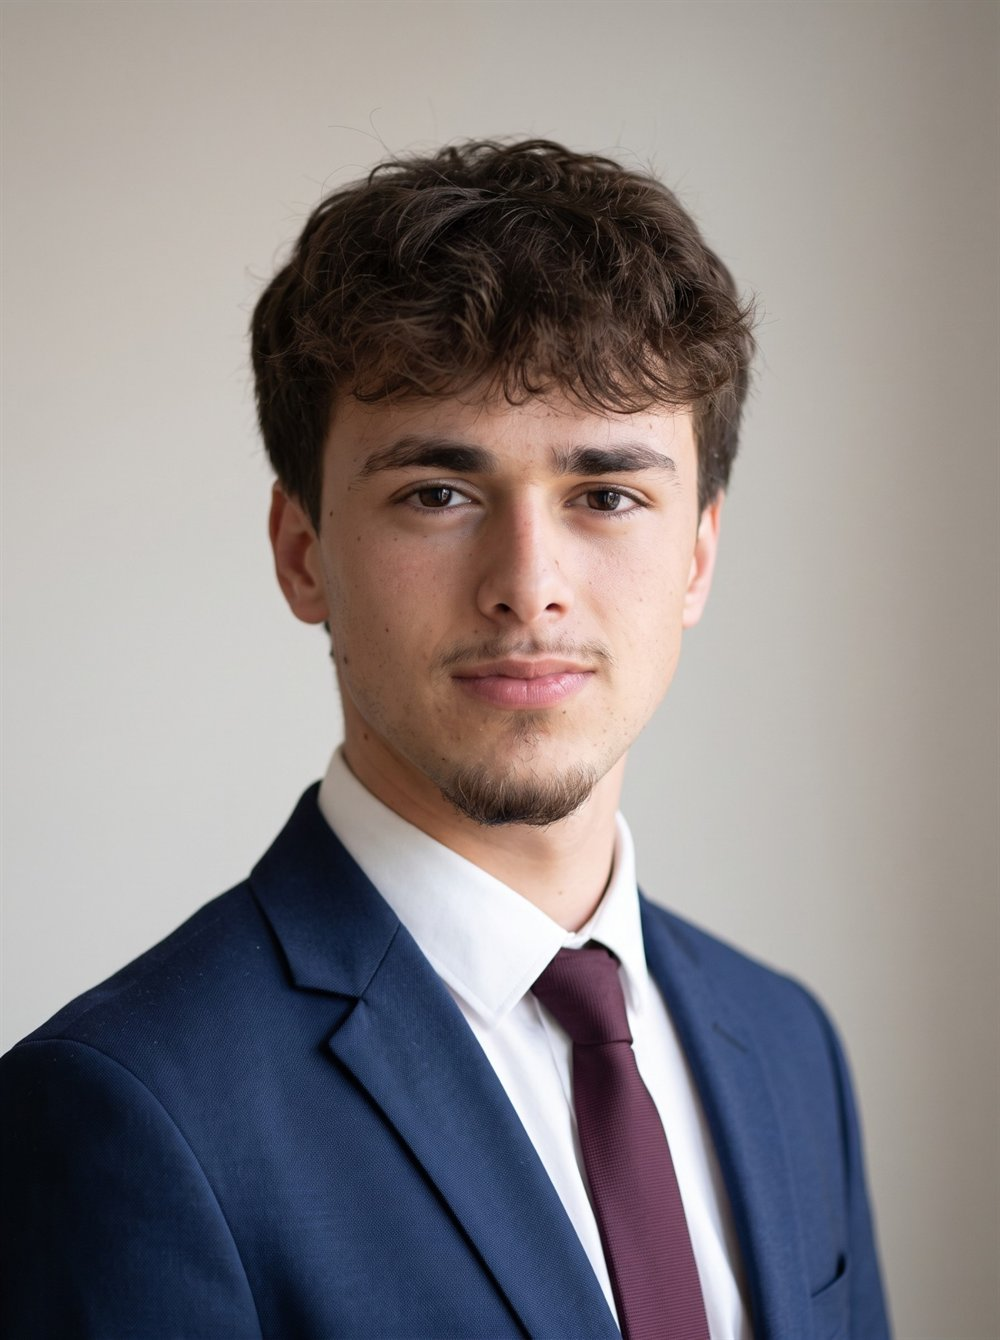
\includegraphics[width=32mm]{robin-canovas.jpg}};
    \end{scope}
    \draw[line width=1.6pt, white] (P) circle (15mm);
    \draw[line width=0.8pt, brandcyan!70] (P) circle (16.4mm);

    % Nom, titre, contact
    \node[anchor=north west, inner sep=0, text=white, font=\fontsize{27}{29}\selectfont]
      at ($(NW)+(50mm,-7.5mm)$) {\cvfirstname\ \textbf{\cvlastname}};
    \node[anchor=north west, inner sep=0, text=brandcyan!45!white, font=\bfseries\normalsize]
      at ($(NW)+(50mm,-18.5mm)$)
      {\tr{Étudiant en informatique en alternance \,·\, Profil généraliste}
          {Computer Science student, work-study \,·\, Generalist profile}};
    \node[anchor=north west, inner sep=0, text=white!78!ink, font=\small]
      at ($(NW)+(50mm,-24mm)$)
      {\tr{Bases de données \,·\, Réseaux \& DevOps \,·\, Mathématiques \,·\, Sécurité}
          {Databases \,·\, Networks \& DevOps \,·\, Mathematics \,·\, Security}};
    \node[anchor=north west, inner sep=0, text=white, font=\small, align=left]
      at ($(NW)+(50mm,-31mm)$) {%
        \contacticon{\hmail}\href{mailto:\cvmail}{\cvmail}\hspace{9pt}
        \contacticon{\hpin}\cvcity\\[3pt]
        \contacticon{\hlinkedin}\href{https://www.linkedin.com/in/\cvlinkedin}{linkedin.com/in/\cvlinkedin}\hspace{9pt}
        \contacticon{\hglobe}\href{https://\cvsite/}{\cvsite}};

    % QR code vers le portfolio
    \node[anchor=north east, fill=white, rounded corners=2pt, inner sep=2pt] (qr)
      at ($(NE)+(-10mm,-8mm)$) {\qrcode[height=17mm]{https://robincanovas.github.io/portfolio/}};
    \node[anchor=north, text=white!75!ink, font=\scriptsize, align=center]
      at ($(qr.south)+(0,-1.5mm)$) {\tr{Portfolio \& démos}{Portfolio \& demos}};
  \end{tikzpicture}%
  \par\vspace*{\dimexpr\headerheight-12mm\relax}}
